% Created 2020-05-25 Mon 14:42
% Intended LaTeX compiler: lualatex
\documentclass[a4paper,12pt,twoside]{report}
\usepackage{graphicx}
\usepackage{grffile}
\usepackage{longtable}
\usepackage{wrapfig}
\usepackage{rotating}
\usepackage[normalem]{ulem}
\usepackage{amsmath}
\usepackage{textcomp}
\usepackage{amssymb}
\usepackage{capt-of}
\usepackage{hyperref}
\usepackage{color}
\usepackage{listings}
\usepackage[a4paper,margin=1cm]{geometry}
\author{Vladimir Nikishkin}
\date{\today}
\title{Figure 1.3 A linear recursive process for computing \(6!\).}
\hypersetup{
 pdfauthor={Vladimir Nikishkin},
 pdftitle={Figure 1.3 A linear recursive process for computing \(6!\).},
 pdfkeywords={},
 pdfsubject={},
 pdfcreator={Emacs 26.3 (Org mode 9.3.4)}, 
 pdflang={English}}
\begin{document}

\maketitle
\tableofcontents

\lstset{numbers=left,frame=single,language=[LaTeX]TeX,label=org47a7ea4,caption= ,captionpos=b}
\begin{lstlisting}
\begin{minipage}{18cm}
\begin{tikzpicture}[color=blue]
\path node[align=left] (0,0) {
(factorial 6)\\
(* 6 (factorial 5))\\
(* 6 (* 5 (factorial 4)))\\
(* 6 (* 5 (* 4 (factorial 3))))\\
(* 6 (* 5 (* 4 (* 3 (factorial 2)))))\\
(* 6 (* 5 (* 4 (* 3 (* 2 (factorial 1))))))\\
(* 6 (* 5 (* 4 (* 3 (* 2 1)))))\\
(* 6 (* 5 (* 4 (* 3 2))))\\
(* 6 (* 5 (* 4 6)))\\
(* 6 (* 5 24))\\
(* 6 120)\\
720};
\path[draw,>->,>={Triangle[open]},thick,rounded corners=30pt] 
(-1cm,2.3cm) .. controls (0cm,2.3cm) and (-0.8cm,2.3cm) .. (4cm, 0.2cm)
 .. controls (-1.6cm,-2.3cm) .. (-2.4cm,-2.3cm );
\end{tikzpicture}
\end{minipage}
\end{lstlisting}

\begin{center}
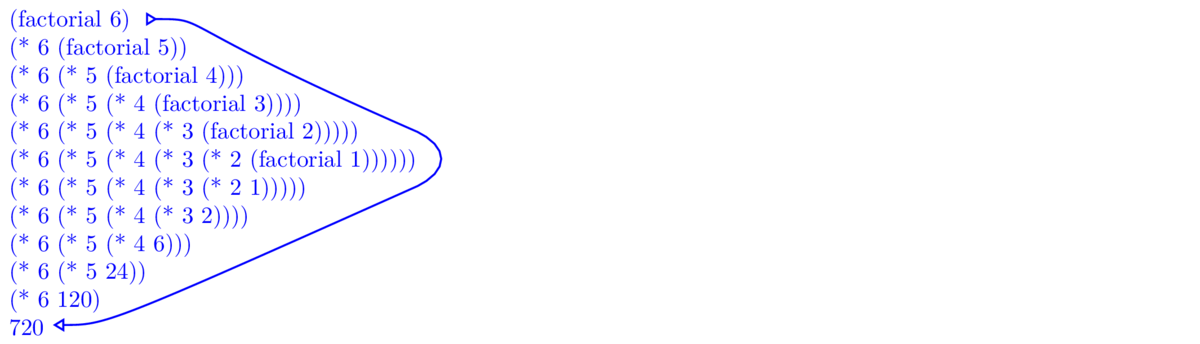
\includegraphics[width=.9\linewidth]{figure-1-3-factorial.png}
\end{center}
\end{document}